\section{Why the models fail on mixed input}
\label{sec:diagnosis}

\begin{figure*}[t]
  \centering
  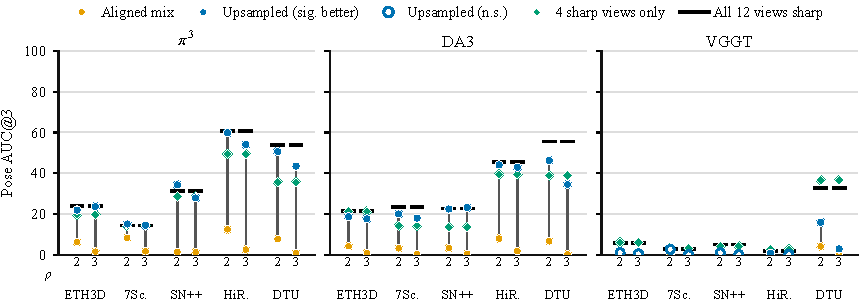
\includegraphics[width=\textwidth]{figures/fig_diagnosis.pdf}
  \caption{\textbf{The diagnosis across all models, datasets and ratios} (pose \auc, 4 sharp + 8 small views, lower token level). For \pithree and \dathree, upsampling the small views (blue) lifts the aligned mix (orange) close to the all-sharp reference (black bar) in every cell, and usually above the 4 sharp views alone (green). For VGGT it does not. Filled blue marks a significant difference between upsampled and aligned.}
  \label{fig:diagnosis}
\end{figure*}

\begin{table}[t]
\centering\small
\setlength{\tabcolsep}{4pt}
\begin{tabular}{@{}lcc@{}}
\toprule
Input (\pithree, HiRoom, $\rho{=}2$) & Pose \auc & F-score \\
\midrule
Mix as-is                        & 0.8  & 0.152 \\
+ positions aligned              & 12.5 & 0.214 \\
+ attention correction           & 17.6 & 0.236 \\
Small views dropped (4 sharp)    & 49.4 & 0.360 \\
Small views upsampled            & 59.8 & 0.699 \\
All 12 views sharp (reference)   & 60.9 & 0.736 \\
\bottomrule
\end{tabular}
\caption{\textbf{One row of the diagnosis.} Upsampling the small views adds no information, yet nearly closes the gap to the all-sharp reference; changes inside the model close little of it. Reconstruction numbers here are from a readout in which not every job had been fused yet (\cref{sec:discussion}).}
\label{tab:teaser}
\end{table}

\subsection{All three models collapse}

\Cref{tab:teaser} follows one setting, \pithree on HiRoom with 8 of 12 views at half resolution, through every intervention. Fed as it is, the mix scores 0.8 \auc against 60.9 when all views are sharp, and its reconstruction F-score drops from 0.736 to 0.152. \dathree falls the same way, from 45.4 to 1.1. VGGT is low with every input at this token level (\cref{fig:teaser}), a point we return to in \cref{sec:vggt}.

The small views are not simply less useful than sharp ones; for pose they can be harmful. When we score only the four sharp frames that every input shares, the aligned mix is below the four sharp views on their own in 28 of 30 pose cells, 17 of them significantly, and significantly above them in one. On the replication seed, dropping the small views again beats the aligned mix on these frames (4/0 for \pithree, 7/0 for \dathree and 4/1 for VGGT). Reconstruction is less one-sided: small views can still add coverage. For \pithree on ETH3D at $\rho{=}2$, the aligned mix reaches an F-score of 0.353 against 0.158 with the sharp views alone.

\subsection{For \pithree and \dathree, the loss is mostly representation}

If the mix fails because small views carry less information, then upsampling them should not help, since it adds none. It helps a great deal. Upsampled small views beat the aligned mix in all 10 pose cells for both \pithree and \dathree (\cref{tab:diag,fig:diagnosis}). The gains are large: $+6.8$ to $+51.5$ \auc for \pithree and $+14.5$ to $+41.0$ for \dathree, and $+0.13$ to $+0.57$ in F-score for \pithree and $+0.12$ to $+0.49$ for \dathree.

To see how much of the loss this recovers, we use the recovery ratio
\begin{equation}
  R \;=\; \frac{\text{up} - \text{aligned}}{\text{true} - \text{aligned}},
  \label{eq:recovery}
\end{equation}
which is 0 when upsampling does nothing and 1 when it matches truly sharp input. For pose, $R$ lies between 80\% and 110\% for \pithree and between 62\% and 102\% for \dathree at the lower token level, and between 87--110\% and 74--104\% at the higher level (\cref{fig:recovery}). Values above 100\% mean the upsampled mix did slightly better than the true sharp input. In other words, giving the small views the same size as the sharp ones recovers most of what was lost, while the information they carry stays the same. For these two models the loss comes mainly from the views being of different sizes, not from what the small views lack.

Real detail does matter at the extremes. The gap between true and upsampled input is concentrated on DTU at $\rho{=}3$, where it is $+10.5$ \auc for \pithree and $+21.1$ for \dathree, and it grows as $\rho$ reaches 4 (\cref{sec:robust}).

\begin{table}[t]
\centering\small
\setlength{\tabcolsep}{2.6pt}
\begin{tabular}{@{}lcccccc@{}}
\toprule
 & \multicolumn{3}{c}{Pose (10 cells)} & \multicolumn{3}{c}{Reconstruction (8 cells)} \\
\cmidrule(lr){2-4}\cmidrule(l){5-7}
First vs second input & \pithree & \dathree & VGGT & \pithree & \dathree & VGGT \\
\midrule
Aligned vs as-is       & 7/0 & 5/0 & 5/0 & 5/0 & 4/0 & 5/0 \\
+Attention vs aligned  & 6/0 & 2/1 & 3/0 & 1/0 & 0/0 & 0/0 \\
Upsampled vs aligned   & \textbf{10/0} & \textbf{10/0} & 3/0 & \textbf{7/0} & \textbf{7/0} & 0/4 \\
Upsampled vs shrunk    & 10/0 & 10/0 & 7/0 & 6/0 & 8/0 & 5/1 \\
True vs upsampled      & 3/0 & 2/0 & \textbf{9/0} & 0/0 & 1/2 & \textbf{7/0} \\
\bottomrule
\end{tabular}
\caption{\textbf{Significant wins/losses of the first input over the second} (4 sharp + 8 small views, $\rho\in\{2,3\}$, lower token level). Pose covers five datasets; reconstruction covers the first four (ETH3D with 9 of 11 scenes). DTU is left out of reconstruction because some of its $\rho{=}3$ inputs have undefined Chamfer distance. VGGT's cells at this level sit close to its floor (\cref{sec:vggt}).}
\label{tab:diag}
\end{table}

\begin{figure}[t]
  \centering
  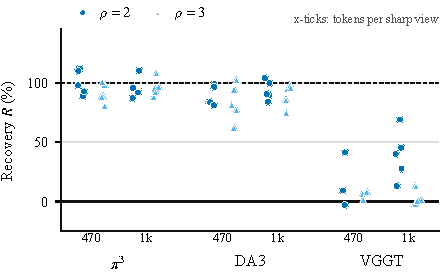
\includegraphics[width=\linewidth]{figures/fig_recovery.pdf}
  \caption{\textbf{Share of the pose loss recovered by upsampling} ($R$, \cref{eq:recovery}), one point per dataset, at two token levels. \pithree and \dathree recover nearly everything at both levels; VGGT does not, even with about 1{,}000 tokens per sharp view. Cells where the all-sharp input beats the aligned mix by less than 3 \auc are omitted, since $R$ is then unstable.}
  \label{fig:recovery}
\end{figure}

\subsection{\dathree rules out positions as the only cause}

Misaligned positions are the obvious suspect. In VGGT and \pithree, a patch of a small view gets a position on its own coarse grid, so in global attention it is compared with sharp-view patches whose positions mean something different. \dathree is a natural control, because its global attention gives every patch the same position. Before running it, we predicted that \dathree would barely degrade on mixed input and that aligning positions would not help it. Both predictions failed. \dathree collapses as hard as the others (1.1 \auc against 45.4 on HiRoom at $\rho{=}2$), and aligning positions, which for \dathree can only act inside frame attention, helps it significantly on all five datasets at $\rho{=}2$. Misaligned positions across views therefore cannot be the whole cause. How many tokens a view has, and how they are spaced, matter within each view as well.

\subsection{VGGT fails differently}
\label{sec:vggt}

VGGT does not follow this pattern. Upsampling beats the aligned mix in only 3 of 10 pose cells, and in reconstruction the aligned mix wins 4 of 8 cells. Real pixels matter instead: true sharp input beats upsampled input in 9 of 10 pose cells and 7 of 8 reconstruction cells.

At the lower token level, VGGT scores close to zero even with all 12 views sharp (on ETH3D at $\rho{=}2$, 5.9 \auc, against 1.0 upsampled), so these cells alone are weak evidence. The higher token level puts VGGT well above that floor: with all views sharp it reaches 54.0 on ScanNet++, against 5.1 at the lower level, and 95.5 on DTU. We predicted that the gap between true and upsampled input would shrink there. It grew in 9 of 10 cells, and upsampling recovers only 13--69\% of the loss at $\rho{=}2$ and between $-3\%$ and 13\% at $\rho{=}3$.

Uneven detail appears to be what hurts VGGT. When all 12 views are blurred to the small views' detail, so that no view is sharper than another, VGGT does better than with 4 sharp and 8 upsampled views in 16 of 20 cells, against 11 of 20 for \dathree and 1 of 20 for \pithree (where the mix wins 2). On ScanNet++ at $\rho{=}2$, the blurred input scores 50.0, close to the 54.0 of all-sharp input, while the sharp-plus-upsampled mix scores 27.3. At $\rho{=}3$ the blur itself costs too much detail (3.9 on the same dataset). VGGT is also far more sensitive to the number of tokens per view: with 10 uniform views on DTU, going from 4{,}096 to 8{,}192 tokens lifts it from 26.2 to 87.2 \auc, against 43.9 to 55.6 for \pithree. VGGT treats its first view as a reference, unlike \pithree, and this is a plausible reason for its behaviour, but we did not test it, and we do not establish why VGGT differs.

\subsection{The diagnosis is robust}
\label{sec:robust}

The picture for \pithree and \dathree holds under every variation we tried, all scored on pose. With splits of 2+10 and 6+6 views, upsampling beats the aligned mix in 20 of 20 cells for both models (VGGT 8 of 20). At $\rho{=}4$ it does so in 10 of 10 for both, and real pixels begin to matter more: the mean gap between true and upsampled input widens from $+2.8$ to $+4.5$ \auc for \pithree and from $+5.6$ to $+9.6$ for \dathree. When the 8 small views come in four sizes ($\mixsize/1.5$, $/2$, $/3$ and $/4$, two views each), upsampling again wins 10 of 10 cells for both models, while for VGGT it wins 1 and loses 2. Finally, we reran the core diagnosis on a new seed, which draws new frames and new sharp views. Of the 189 cells that are significant on both seeds, 188 agree in direction and one flips. On HiRoom at $\rho{=}2$, \pithree's ladder on the new seed reads 0.9 as-is, 9.1 aligned, 57.3 upsampled and 62.7 all-sharp, against 0.8, 12.5, 59.8 and 60.9 on the reporting seed.
